\documentclass[letterpaper,12pt]{article}

\usepackage{graphicx}
\graphicspath{{./images/}}
\usepackage{amssymb}
\usepackage{amsmath}
\usepackage{amstext}
\usepackage{subfigure}
\usepackage[framed]{mcode}
\usepackage{url}
\usepackage{color}
\usepackage{hyperref} \hypersetup{pdfborder={0 0 0}}
\usepackage{verbatim}

\addtolength{\oddsidemargin}{-.875in}
\addtolength{\evensidemargin}{-.875in}
\addtolength{\textwidth}{1.75in} \addtolength{\topmargin}{-.875in}
\addtolength{\textheight}{1.75in} \special{papersize=\the\paperwidth,\the\paperheight}

\begin{document}

\begin{table}[h]
\begin{tabular}{cc}
  
\includegraphics[width=2in,keepaspectratio=true]{images/logo.eps} &
  \begin{tabular}{c}
    \vspace*{0.5cm}{\large ECE4305: Software-Defined Radio Systems and Analysis} \\
    \vspace*{0.1cm}{\large Laboratory 0: Introduction To SDR} \\
  \end{tabular}\\
  \hline
\end{tabular}
\end{table}

\section*{Objective} This laboratory will introduce the concept of a communication systems and introduce channel noise. Specifically, a simplified error model will be discussed along with the theoretical connections to random processes discussed in Chapters III and IV. Moreover, MATLAB\textregistered~ will also be introduced as development tools for digital communication systems, especially the construction of a prototype software-defined radio (SDR) based simulation. An overview of the PLUTO radio will also be provided.
\tableofcontents

\newpage

\section{Theoretical Preparation}
The fundamental concepts of digital communication systems and related theoretical background material covered in this section will serve as a basis for the implementation and design of prototype systems throughout the rest of this course.

\subsection{Connection To Theory}
\begin{comment}
A common communication system model consists of three basic components: transmitter, channel, and receiver.  Where the transmitter is responsible for symbol generation, the channel performs some corruption upon these symbols, and the receiver recovers these corrupted symbols.  In this lab we will be considering the channel as only a noise source to the system, but will consider more complicated models in future labs.\par
%
When we consider the performance of a communication link, in the most basic sense, we are interested in the bandwidth and power of the transmitted signal. Bandwidth is measured from the power spectral density of signal and is also proportional to the bit rate. In Chapter 4, we defined average energy per bit as:
%
\begin{equation}
    \bar{E}_b = \frac{\bar{E}_s}{\bar{log_2(M)}}
\end{equation}
%
where $M$ is the order of the modulation scheme and $\bar{E}_s$ is the average symbol energy. Note that $\bar{E}_b$ is of units Joules/bit. When considering an Additive White Gaussian Noise (AWGN) channel, we can write the power efficiency as $\bar{E}_b/N_0$, where $N_0$ is the noise power spectral density (PSD). Since AWGN is flat in frequency, or equal across all frequencies, channel noise can typically be measured over $1$ Hz of spectrum.  Therefore, $N_0$ is in units Watts/Hz $\rightarrow$ Joules. $\bar{E}_b/N_0$ can be alternatively understood as normalized signal-to-noise ratio (SNR) and is related by the bitrate $R_b$ and channel bandwidth $B$
%
\begin{equation}\label{SNR}
    SNR = \frac{\bar{E}_b}{N_0}\times\frac{R_s}{B}.
\end{equation}
%
SNR is commonly expressed in SNR in decibels (dB) and Equation~\eqref{SNR} can be rewritten as:
%
\begin{equation}
    SNR_{dB} = 10\,log_{10}(\bar{E}_b/N_0) + 10\,log_{10}(R_s/B)
\end{equation}
%
When determining SNR of a signal it is important to understand that signals are band limited unlike noise.  Therefore, as the observation bandwidth of the signal is increased the SNR becomes worse.

\subsection{Noise Generation and Signal-To-Noise Ratio}\end{comment}
%
Calculation of power is a non-trivial exercise in practice and in many situations loosely defined. This is especially true when determining SNR. Let us first consider a unique example where we have scaled exponentials ($s(t) = \alpha\,exp(j\pi f_c t)$) in AWGN. A resulting FFT provided in Figure~\ref{fig:snr_guess} generated from some simple code for two different source signals:\par
%
\begin{minipage}{\linewidth}
\begin{lstlisting}
  r = signal+noise;
  % View averaged spectrum
  freq = linspace(-bandwidth/2,bandwidth/2,fftLen);
  R = reshape(r,fftLen,frames);
  R = fftshift(fft(R));
  R_mean = mean(abs(R),2)/fftLen;
  plot(freq,10*log10(R_mean));
\end{lstlisting}
\end{minipage}
%
\begin{figure}[htp!]
\centering
\includegraphics[width=0.75\textwidth]{snr_guess_dual.eps}
\caption{Averaged FFT of two different received signals with identical noise.}\label{fig:snr_guess}
\end{figure}
%
\par An obvious question to ask would be ``What is the SNR of these signals?''.  However, we cannot directly derive the SNR from this plot alone.  If we are using a spectrum or vector analyzer we need knowledge of the Resolution Bandwidth (RBW), which is a function of the FFT bin count and observation bandwidth. Since we already know the observation bandwidth ($1$ MHz), if we used a FFT of size 1024, then the true SNR is $\sim 10$ dB. An important aspect to note from Figure~\ref{fig:snr_guess} is the shape of the signals $r_1$ and $r_2$. In generation these two signals only differ in $f_c$, although they appear quite different in the figure. $r_2$ was strictly chosen to be within a FFT bin and $r_2$ strattles bins. This difference is due to the window effect of the FFT applied to the signals. This is commonly known as \textit{scalloping} and will be dependent on the window chosen. fred harris (yes that capitalization is correct) provides a detailed overview of different windows and how to compensate for their effects in~\cite{harris1978}. When performing digital signal processing it is alway important to understand effects of discrete computations over the infinite resolution of our written equations.\par
%
Now let us connect this to the theoretical concepts provided in the lectures and book. From Section 3.3.4 in the textbook we know that the power spectral density (PSD) is obtained through a Fourier Transform of a signal's autocorrelation function. Formally written as:
%
\begin{equation}
S_{XX}(f) = \int_{-\infty}^{\infty} \! R_{XX}(\tau)e^{-j2{\pi}f\tau}
\, d\tau
\end{equation}
%
where the autocorrelation of our process or signal $X(t)$ is:
%
\begin{equation}
\begin{split}
    R_{XX}(t_1,t_2)&=E[X(t_1)X^{\ast}(t_2)].
\end{split}
\end{equation}
%
In the case of AWGN this autocorrelation is simply:
%
\begin{equation}
  R_{XX}(t_1,t_2) =
  \begin{cases}
    \sigma^2 & \text{if $t_1=t_2$} \\
    0        & \text{otherwise}
  \end{cases}
\end{equation}
%
where $\sigma^2$ is the variance of the noise.  Therefore, $S_{XX}=\sigma^2$ for all frequencies within the observation bandwidth. and the power of the AWGN signal is simply $P_N = \sigma^2\times B$. This result provides a mechanism for determining power from the PSD or frequency domain of a signal.  However, it can be useful to calculate signal power from the time domain, and from Parseval's theorem we know power is identical between domains.  For an AWGN signal calculating the variance directly provides $P_N$, but this is not true for non-zero mean processes.  In that case, power can be simply calculated based on the squared RMS or squared mean of the process samples. However, a significant amount of data should be collected to get a representative power value of the signal.\par
%
To generate white noise with a specific PSD in MATLAB is a straight-forward process, but we need to be cautious of our units and concepts of time since time is abitrary in MATLAB. We will walk through a simple example where we generate white noise both complex and real for a given PSD and bandwidth. If we are given a specification sheet of a RF product it should provide one of two values: noise power over a given bandwidth (Usually defined at DANL), or possibly average PSD over a given band.  When noise PSD numbers are given they are usually provide in dBm/Hz, which is what we will use here.  Provided in the lab is script \textit{generateNoise.m} which is also provided in the Figure below.\par
%
\begin{figure}[!htp]
    \centering
\begin{minipage}{0.9\linewidth}
\begin{lstlisting}
    %% Generate noise and calculate Noise Power
    % Choose parameters
    noiseFloorDBMHZ = -30; % dBm/Hz
    bandwidth = 1e6; % Hz (-bandwidth/2 -> bandwidth/2)
    % Convert to linear units
    noiseFloorWHZ = 10^((noiseFloorDBMHZ-30)/10); % Watts/Hz
    % Calculate noise power
    NoisePower = noiseFloorWHZ*bandwidth; % Watts
    % Generate AWGN signal with desired noise power
    fftLen = 2^10; frames = 1e3;
    noiseC = sqrt(NoisePower)/sqrt(2).*...
        (randn(fftLen*frames,1)+randn(fftLen*frames,1).*1i); % Complex noise
    noise = sqrt(NoisePower).*(randn(fftLen*frames,1)); % Real Noise
    % Check
    disp([NoisePower var(noise) var(noiseC) rms(noise)^2 rms(noiseC)^2]);

    %% Veryify PSD
    noiseFramesC = reshape(noiseC,fftLen,frames);
    noiseFrames = reshape(noise,fftLen,frames);
    % Determine PSD in Watts/(Frequency Bin)
    noiseFramesFreqC = fft(noiseFramesC,fftLen);
    noiseFramesFreq = fft(noiseFrames,fftLen);
    % Autocorrelate and calculate mean power
    S_kC = mean(abs(noiseFramesFreqC).^2,2)/fftLen;
    S_k = mean(abs(noiseFramesFreq).^2,2)/fftLen;
    % Convert to dBm/Hz
    S_k_DBMHZC = 10*log10(S_kC/bandwidth) + 30;
    S_k_DBMHZ = 10*log10(S_k/bandwidth) + 30;
    % Plot
    freqs = linspace(-bandwidth/2,bandwidth/2,fftLen);
    figure;plot(freqs,S_k_DBMHZ,freqs,S_k_DBMHZC);
    xlabel('Hz');ylabel('dBm/Hz');grid on;
    ylim(noiseFloorDBMHZ+[-20 20]);
    legend('Real Noise','Complex');

\end{lstlisting}
\end{minipage}
\caption{MATLAB code for generating white noise from specific PSD metric.}\label{fig:power_code}
\end{figure}
%
There are three important ideas that should be pointed out in this script.  First, when generating noise from \texttt{randn} it is scaled to maintain unit magnitude.  Second, two different ways are provided to determine the power of the noise of the generated signal using both the \texttt{var} and \texttt{rms} functions. Finally, when verifying the PSD of the produced signal we simply utilize the direct Einstein-Wiener-Khinchin (EWK) relation as discussed above.\par
%
Within MATLAB there are also several other tools that can be used to generate PSDs of signals such as \texttt{pwelch}, \texttt{periodogram}, and \texttt{pmtm} among others.  When using make sure you understand their parameterization, since these function can be rather complex. However, they can provide more useful results beyond the simple application of EWK used above.

\begin{itemize}
  \item Question 0: What is the SNR in dB for the red signal of Figure~\ref{fig:snr_guess} if the resolution bandwidth is reduced by half?
  \item Question 1: Generate a complex noise signal with $100\,\,\mu$Watts of power and provide a PSD plot (in dBm/Hz) over $1$ MHz of bandwidth.
  \item Question 2: Generate a sinusoidal signal with power $0$ dB of power and provide a PSD plot (in dBm/Hz) over $1$ MHz of bandwidth.
  \item Question 3: Calculate the SNR of the signals and noise from Questions 1 and 2 over $500$ kHz of bandwidth.
\end{itemize}

\subsection{Complex Baseband \& Signal Representation}
Understanding how a signal is represented can greatly enhance one's
ability to analyze and design baseband digital communication
systems. We need a convenient
mathematical framework to represent signal and noise. We usually have two: Envelope/Phase and In-phase/Quadrature.\\

\noindent
A bandpass signal can be represented by the sum of its in-phase (I) and quadrature (Q) components:
\begin{equation}
x(t) = R_{I}(t)\cos{(2{\pi}f_{c}t)}-R_{Q}(t)\sin{(2{\pi}f_{c}t)}.
\end{equation}
where $R_{I}(t)$ is in-phase amplitude, $R_{Q}(t)$ is quadrature amplitude and $f_{c}$ is carrier frequency.
It can also be represented as a sinusoid by its envelope and phase:
\begin{equation}
x(t) = R(t)\cos{({\omega}t+{\phi}(t))},
\end{equation}
where $R(t)$ is the amplitude and ${\phi}(t)$ is phase offset.\\

\noindent Consider a 4-QAM signal constellation and how it would be
represented by I and Q or its envelope and phase. If you needed to
compute the distance between two points, which representation would
be easier to work with?  What about with other signal
constellations?  Table~\ref{signaltable} shows these relationships
graphically.\\

\begin{table}[htp]
\centering
\caption{Signal representations of ${A}\sin(\omega t+{\phi}$).}
\begin{tabular}{|c|c|c|}
\hline
&Envelope/Phase&In-phase/Quadrature\\
&$\mathbf{A,\phi}$ & $\mathbf{(A\sin\phi),(A\cos\phi)}$\\
\hline
{Time}& {$\mathbf{A}\sin(\omega t+\mathbf{\phi})$} & $\mathbf{(Acos\phi)}\sin(\omega t)$ \\
 & & $ + \mathbf{(Asin\phi)}\cos(\omega t)$\\
\hline
Waveform& {\includegraphics[width=150pt]{./1.eps}}& 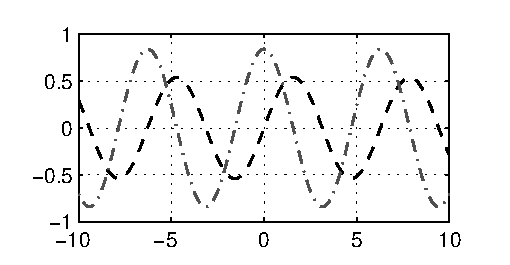
\includegraphics[width=150pt]{./2.eps}\\
\hline
Vector&
\includegraphics[width=100pt]{./3.eps} &
\includegraphics[width=100pt]{./4.eps} \\
\hline
\end{tabular}
\label{signaltable}
\end{table}

\noindent
Given the importance of representing signals in an efficient format, consider how you would compute the distance between two constellation points in QPSK whose four
points given in I/Q format are:
\begin{displaymath}
\centering
S_{1}(t) = +A\cos{(2{\pi}f_{c}t)}+A\sin{(2{\pi}f_{c}t)},
\end{displaymath}
\begin{displaymath}
\centering
S_{2}(t) = -A\cos{(2{\pi}f_{c}t)}+A\sin{(2{\pi}f_{c}t)},
\end{displaymath}
\begin{displaymath}
\centering
S_{3}(t) = -A\cos{(2{\pi}f_{c}t)}-A\sin{(2{\pi}f_{c}t)},
\end{displaymath}
\begin{displaymath}
\centering
S_{4}(t) = +A\cos{(2{\pi}f_{c}t)}-A\sin{(2{\pi}f_{c}t)}.
\end{displaymath}
Using basic trigonometry, the distance between any two points can be quickly computed using the law of cosines, namely:
\begin{equation}
C^2 = A^2 + B^2 - 2ABcos(\theta).
\label{eq:lawcosines}
\end{equation}
This solution yields the distance between the two points.  The same principle holds true for other signal constellations including M-QAM, M-PSK, M-PAM,
7-around-1, BOX, etc.  Although the trigonometry can be different for various constellations, it is almost always simpler to evaluate the math if you represent the signals in complex baseband.

\subsection{Suggested Readings}
Although this laboratory handout provides some information about the fundamentals of digital communications, the reader is encouraged to review the material from the
following references in order to gain further insight on these topics.
\begin{itemize}
 \item Overview of Signals and Systems:
\begin{itemize}
 \item Chapter 2 in Reference~\cite{rice2009}.
\end{itemize}
 \item Overview of Probability Theory:
\begin{itemize}
 \item Chapter 4 in Reference~\cite{rice2009}.
\end{itemize}
 \item Introduction to Communication Simulation Techniques:
\begin{itemize}
 \item Chapter 1 in Reference~\cite{silage2009}.
\end{itemize}
\end{itemize}

\clearpage
% \subsection{Problems}
% \begin{enumerate}
% \item{
% The power spectral density of a narrowband noise signal, $n(t)$, is shown in Figure \ref{fig:problem1}. The carrier frequency is 10~Hz.
% \begin{enumerate}
% \item{Find the power spectral densities of the in-phase and quadrature components of $n(t)$}.
% \item{Find their cross-spectral densities.}
% \end{enumerate}
% \begin{figure}[ht]
% \centering
% 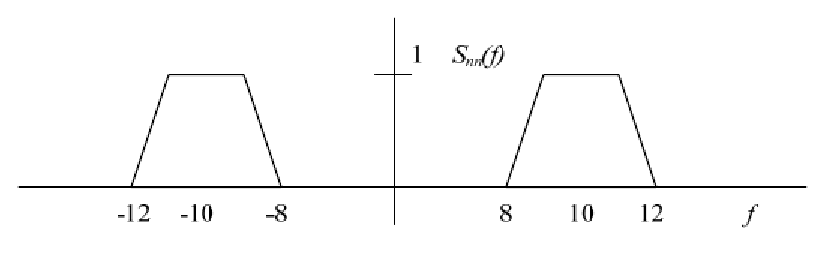
\includegraphics[scale=0.7]{problem1.eps}\\
% \caption{Power spectral density of a narrowband noise signal, $n(t)$.}\label{fig:problem1}
% \end{figure}
% }
% \item{
% The input to a time-invariant linear system with impulse response $h(t)$ is a white Gaussian noise process $X(t)$ with two-sided spectral density $N_{o}\over{2}$.  The output is the random process $Y(t)$.  The filter's response is given in terms of $p_T(t)$, the rectangular pulse of duration $T$, by $h(t) = {sin(2{\pi}t)\over{T}} * p_T(t)$.
% \begin{enumerate}
% \item{Find the cross-correlation function $R_{X,Y({\tau})},-{\infty} < \tau < \infty$.}
% \item{Find $R_{Y}(0)$.}
% \end{enumerate}
% }
% \item{
% Prove the following two properties of the autocorrelation function $R_{X}(\tau)$ of a random process $X(t)$:
% \begin{enumerate}
% \item{If $X(t)$ contains a DC component equal to $A$, then $R_{X}(\tau)$ will contain a constant component equal to $A^2$.}
% \item{If $X(t)$ contains a sinusoidal component, then $R_{X}(\tau)$ will also contain a sinusoidal component of the same frequency.}
% \end{enumerate}
% }
% \item{
% Consider a pair of stationary processes $X(t)$ and $Y(t)$. Show that the cross-correlations $R_{XY}(\tau)$ and $R_{YX}(\tau)$ of these processes have the following properties:
% \begin{enumerate}
% \item{$R_{XY}(\tau)=R_{YX}(-\tau)$}
% \item{$|R_{XY}(\tau)|\leq\frac{1}{2}[R_{X}(0)+R_{Y}(0)]$}
% \end{enumerate}
% }
% %\item{
% %Find and compare the power spectral efficiency for the three binary signal sets below.  Give the relative performance in dB.  Assume the \emph{$s_{1}(t)$} and \emph{$s_{2}(t)$} are equally likely.
% %\begin{enumerate}
% %\item{$s_{1}(t) = Bsin({\omega}_{0}t+\phi)$ and $s_{2}(t) = Bsin({\omega}_{0}t-{\phi})$ for $0{\leq}t{\leq}T$ and where $\bar{E}_{b}{\leq}{A^2T\over{2}}$.  Find the best (\emph{$B,\phi$}).}
% %\item{$s_{1}(t) = Asin({\omega}_{0}t+\theta)$ and $s_{2}(t) = Bsin({\omega}_{0}t)$ for $0{\leq}t{\leq}T$ and where $\bar{E}_{b}{\leq}{A_{0}^2T\over{2}}$ and $A_{0}$ is known.  Find the best (\emph{$A,B,\theta$}).}
% %\item{$s_{1}(t) = Asin({2{\pi}f}_{0}t+{\Delta}t)$ and $s_{2}(t) = Acos({2{\pi}f}_{0}t-{\Delta}t-{\theta})$ for $0{\leq}t{\leq}T$.  Find the best peak frequency deviation, \emph{$\Delta$}, in terms of \emph{T}}.
% %\end{enumerate}
% %}
% \item Exercise~2.21 from the course textbook~\cite{rice2009}.
% \item Exercise~2.53 from the course textbook~\cite{rice2009}.
% \item Exercise~4.1 from the course textbook~\cite{rice2009}.
% \item Exercise~4.3 from the course textbook~\cite{rice2009}.
% \item Exercise~4.6 from the course textbook~\cite{rice2009}.
% \item Exercise~4.7 from the course textbook~\cite{rice2009}.
% \item Exercise~4.26 from the course textbook~\cite{rice2009}.
% \item Exercise~4.27 from the course textbook~\cite{rice2009}.
% \end{enumerate}

\section{Radio Setup and Environmental Noise Observations}

In these laboratory experiments an Analog Devices ADALM-PLUTO SDR with AD9363 transceiver will be used. This SDR in the most basic sense is a System-on-Chip (SoC) with an attached RF module providing complex baseband data. The MATLAB interface utilize the libiio kernel driver to talk with the SDR through a MATLAB class called \texttt{iio\_sys\_obj\_matlab}. The two system objects provided in the hardware support package (HSP) for PlutoSDR
are:
\begin{itemize}
\item comm.SDRRxPluto: PlutoSDR Receiver System object
\item comm.SDRTxPluto: PlutoSDR Transmitter System object
\end{itemize}
These objects are typically constructed through the \texttt{sdrr}x or \texttt{sdrtx} function calls as in Code~\ref{codepluto}.


%
\begin{figure}[!htp]
    \centering
\begin{minipage}{0.5\linewidth}
\begin{lstlisting}
    rx = sdrrx('Pluto')
	tx = sdrtx('Pluto')
\end{lstlisting}
\end{minipage}
\label{codepluto}
\end{figure}

However, these objects can also be directly instantiated directly. The resulting object of sdrrx either
way will have the following basic properties, which will be directly printed to the terminal when not
using the semicolon as:

\begin{figure}[!htp]
    \centering
\begin{minipage}{0.5\linewidth}
\begin{lstlisting}
	rx = sdrrx('Pluto')
	rx =
		comm.SDRRxPluto with properties:
		DeviceName: 'Pluto'
		RadioID: 'usb:0'
		CenterFrequency: 2.4000e+09
		GainSource: 'AGC Slow Attack'
		ChannelMapping: 1
		BasebandSampleRate: 1000000
		OutputDataType: 'int16'
		SamplesPerFrame: 3660
		ShowAdvancedProperties: false
\end{lstlisting}
\end{minipage}
\label{codepluto2}
\end{figure}

The transmitter System object \texttt{comm.SDRTxPluto} has near identical properties except for \textit{GainSource}, \textit{SamplesPerFrame}, and \textit{OutputDataType} which do not make sense in the transmitter context. If you want to examine the available parameters simply type \textbf{doc comm.SDRRxPluto} or \textbf{doc comm.SDRTxPluto} into the MATLAB command prompt.\par
%
Before moving further with the radio it is important to outline how the radio works from the perspective of MATLAB using the \texttt{sdrrx} and \texttt{sdrtx} objects. After an object associated to the SDR has been created, the necessary methods can be run.  

When configured in receive mode and the received method is called, with help from the driver, temporary buffers are created of size \textit{SamplesPerFrame}, as set by the class parameter. Then the device will proceed to fill these buffer with contiguous data from the ADCs. 


For each receive chain there are technically two ADCs, one for the in-phase portion of the signal and one for the quadrature. This is the reasoning behind the multiple buffers.  However, these ADCs are time aligned and sampling of the dual chains happens at the same instances in time.  Once the buffers are filled that data is provided to MATLAB and the link between the device and MATLAB is halted.  As a result, when the receive method is called again from MATLAB the resulting buffer will be disjoint in time from the preceding buffer. For the overall structure of this communication Analog Devices provides a block diagram presented in Figure~\ref{fig:libiio}. The \texttt{PlutoSDR} class for convenience provides the output in a single complex vector, and accepts complex vectors as well.\par
%
\begin{figure}[htp!]
\centering
\includegraphics[width=0.85\textwidth]{sys_obj.png}
\caption{Structure of libiio and SDR hardware interconnection with MATLAB software~\cite{libiio}.}\label{fig:libiio}
\end{figure}
%
Within the FMCOMMS/AD9361 direct downconversion is used to translate signals from RF to baseband frequencies. This is different than traditional heterodyne designs which utilize intermediate frequencies. Therefore, all observed signals passed to MATLAB are at baseband which were originally centered around \textit{CenterFrequency} with a bandwidth of \textit{BasebandSampleRate} parameterized by the \texttt{sdrrx} object.
%
\subsection{Signal Loopback}
%
Now that we have a basic understanding of how the radio operates and have it setup we can perform some simple experiments.
First we will run a simple loopback test which transmits a sinusoidal tone out the transmitter and is simultaneously received at the receiver. To perform this we will utilize the provided \texttt{loopback.m} script.  This script collects multiple buffers of data, which can be necessary since there is an unknown startup lag for the transmitter and the desired signal can be missed. This script should generate a plot similar to the one shown in Figure~\ref{fig:loopback}.
%
\begin{figure}[htp!]
\centering
\includegraphics[width=0.75\textwidth]{loopback.eps}
\caption{Looped back sinusoid observed from the Pluto receiver.}\label{fig:loopback}
\end{figure}
%
%
\begin{itemize}
  \item Modify the amplitude of the sinusoid, along with the PLUTO's \textit{GainSource} and observe their effects.
\begin{itemize}
  \item The three \texttt{GainSource} (AGC) settings are: \textit{Manual}, \textit{AGC Slow Attack}, and \textit{AGC Fast Attack}.
  \item When \textit{Manual} is selected another option called \textit{Gain} becomes available and this parameter can be modified.
  \item It maybe useful to use signals with varying amplitudes or zeros.
  \item If enough gain is applied the sinusoid should appear as a square wave at the receiver.
\end{itemize}
\end{itemize}
%

\subsection{IEEE~802.11 Wireless Local Area Networks}
Another interesting experiment is using the PLUTO to observe the spectrum of wireless local area networks within the vicinity (WLANs).
Most high population density areas employs numerous wireless communication networks for a variety of applications, such as the WPI wireless network.
Consequently, you can use your PLUTO experimentation platform to plot their magnitude spectrum.
IEEE~802.11~\cite{wikipedia_ieee802.11} is one type of WLAN standard that possesses a list of carrier frequencies for a collection of Wi-Fi channels.
For example, The IEEE~802.11 standard
defines Channel~1 of the 2.4~GHz band to be centered at 2.412~GHz.

\begin{itemize}
 \item Specify the \textit{CenterFrequency} parameter of \texttt{sdrrx} with this carrier frequency, use the \texttt{FFTs} or \texttt{dsp.SpectrumAnalyzer} objects to plot their magnitude spectrums.
 \item Since your AD9364 transceiver supports the 6~GHz band as well, also use the \texttt{dsp.SpectrumAnalyzer} to plot spectrum in the 5~GHz band.
\end{itemize}

\noindent
You might want to turn on ``Spectral Averaging'' or ``PlotMaxHoldTrace'' and adjust the amplitude,
since the peaks of these wireless signals could be rather low. It might also be useful to change the \textit{BasebandSampleRate} parameter of \texttt{sdrrx} to adjust the frequency resolution for a better graph of the spectrum.


\subsection{Measurements and the Radio}

What a SDR device like the PLUTO does is give you digital samples. What these are is nothing more or less than what the ADC makes out of the voltages it observes. Then, those numbers are subject to the receiver processing chain which includes frequency translation (Mixing), decimation and filtering.  Analog Devices provides a great overview here ~\cite{ad936x} for the \textit{ad936x}.  Altogether, the complex signal's envelope coming from the PLUTO should be proportional to the voltages observed by the ADC. Therefore, the magnitude square of these samples should be proportional to the signal power as seen by the ADC. However, it must be stress that these are in relation to the range of the ADC. Therefore, these values are of an arbitrary measure relative to the full scale of the ADC and the remaining receive chain, commonly denoted as dBFS~\cite{sigpow}. Scopes provided by MATLAB may denote the signal amplitude in dB but this is just an arbitrary engineering unit.\par
%
With this knowledge we cannot directly determine power of an input signal to the SDR, unless we have performed some calibration and can relate individual samples to received energy. However, SNR can still be determined since signal and noise we be subjected to the same ADC effects and receive chain.  This can be done with techniques already presented previously. For Figure~\ref{fig:snr_test} we again used the transceiver setup, but transmitted signal vectors which contain half zeros and half signal.  After extracting the noise and signal plus noise sections the SNR can be manually calculated simply by:
%
\begin{equation}
    SNR_{dB} = 10\,log_{10}\Big(\frac{P_{SN}-P_{N}}{P_{N}}\Big)
\end{equation}
%
\begin{itemize}
 \item Repeat this process for different \texttt{GainSource} settings and different source amplitudes by modifying the supplied \texttt{loopback.m} script.  Comment on the changes in SNR.
 \end{itemize}
This is a rough method for estimating SNR, but does provides a reasonable metric without additional equipment. To provide better results we would need to remove some of the adaption performed in the receiver conditioning the samples.
%
\begin{figure}[htp!]
\centering
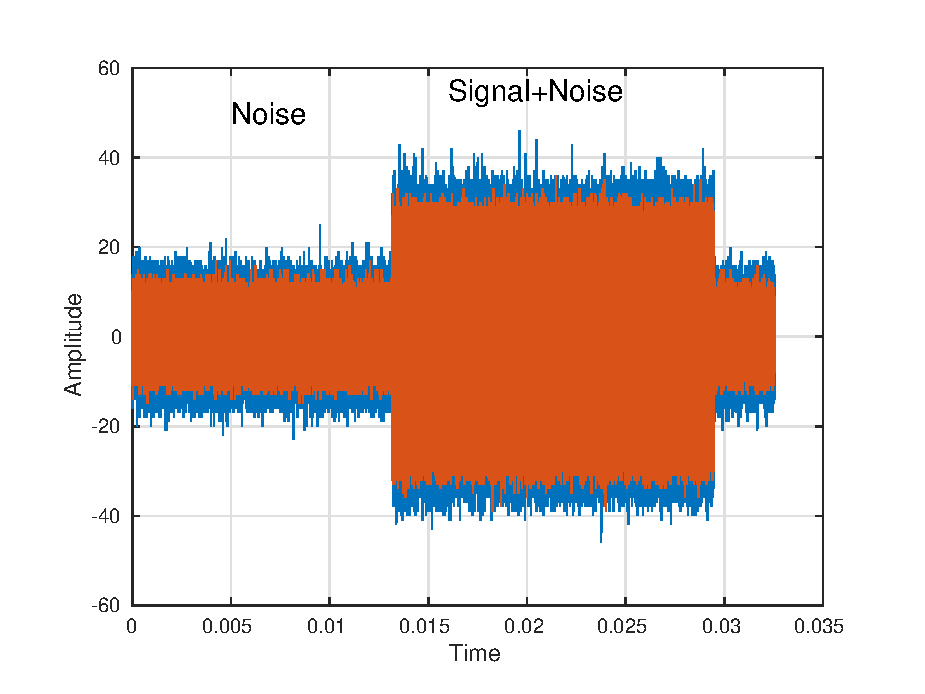
\includegraphics[width=0.75\textwidth]{snr_compare.eps}
\caption{Receive loopback signal with signal half nulled.}\label{fig:snr_test}
\end{figure}

\begin{comment}
\subsection{Random Variables}
A random variable (RV) is a number assigned to every outcome of an experiment. This number could be the gain in a game of chance, the voltage of a random source, the
cost of a random component, or any other numerical quantity that is of interest in the performance of the experiment.\\

\noindent
A random variable is a mapping function whose domain is a sample space and whose range is some set of real numbers:
\begin{equation}
X = X(s)
\end{equation}
where $X$ is the RV and $X(s)$ is the outcome of an experiment.  The cumulative distribution function (CDF) describes how the RV behaves probabilistically,
and is defined as~\cite{Papoulis2002}:
\begin{equation}
F_{x}(x) = P(X{\leq}x).
\label{eq:define}
\end{equation}
Eq.~(\ref{eq:define}) describes the probability that the outcome of an experiment described by the RV $X$ is less than or equal to the dummy variable $x$.\\

\noindent
Several fundamental characteristics of the CDF include the following:
\begin{itemize}
\item{$F_{x}(x)$ is bounded between zero and one.}
\item{$F_{x}(x)$ is a non-decreasing function, i.e., $F_{x}(x_{1}){\leq}F_{x}(x_{2})$} if $x_{1} \leq x_{2}$.
\end{itemize}
The probability density function (PDF) is the derivative of the CDF in terms of the dummy variable $x$, which we can define as~\cite{Papoulis2002}:
\begin{equation}
f_{x}(x) = {d\over{dx}}F_{x}(x).
\end{equation}
For more information about random variables, please refer to Section 4.1 of the course textbook \cite{rice2009}.

\subsection{Central Limit Theorem}
In probability theory, the central limit theorem (CLT) states
conditions under which the mean of a sufficiently large number of
independent random variables, each with finite mean and variance,
can be approximated by a Normal (i.e., Gaussian) distribution. The
CLT also requires the random variables to be identically
distributed. Since real-world quantities are often the balanced sum
of many unobserved random events, this theorem provides a partial
explanation for the
prevalence of the normal probability distribution.\\

\noindent The CLT states that if  you have a set of random variables
${\{}X_{i}{\}}_{i-1}^{i=N}$ such that $X_{i}$ is independently and
identically distributed (i.i.d.), i.e.:
\begin{itemize}
\item{$X_{i}$ are statistically independent.}
\item{$X_{i}$ have the same pdf with mean ${\mu}_{x}$ and variance ${\sigma}_{x}^2$.}
\end{itemize}
Then as $N \rightarrow \infty$, the distribution of the sample expectation will be Gaussian regardless of the original distribution.

\subsection{Gaussian Processes}
In probability theory and statistics, a Gaussian process is a
stochastic process whose realizations consist of random values
associated with every point in a range of times (or of space) such
that each such random variable has a normal distribution. Moreover,
every finite collection of those random variables has a multivariate
normal
distribution.\\

\noindent Gaussian processes are important in statistical modeling
because of properties inherited from the normal distribution. For
example, if a random process is modeled as a Gaussian process, the
distributions of various derived quantities can be obtained
explicitly. Such quantities include the average value of the process
over a range of times, and the error in estimating the average using sample values at a small set of times.\\

\noindent
Given the following expression:
\begin{equation}
y = \int_0^T \! g(t)X(t) \, dt
\end{equation}
we can say that $X(t)$ is a Gaussian process if:
\begin{itemize}
\item{$E(y^2)$ is finite, i.e., does not blow up.}
\item{$Y$ is Gaussian-distributed for every $g(t)$.}
\end{itemize}
Note that the RV $Y$ has a Gaussian distribution, where its PDF is defined as:
\begin{equation}
f_{y}(y) = {1\over{\sqrt{2{\pi}{\sigma}_{y}^2}}}e^{-(y - {\mu}_{y})^2\over{2{{\sigma}_{y}}^2}},
\end{equation}
where ${\mu}_{y}$ is the mean and ${{\sigma}_{y}}^2$ is the variance.  Such processes are important because they closely match the behavior of numerous
physical phenomena, such as additive white Gaussian noise (AWGN).

\subsection{The Q Function}
The Q function is a convenient way to express right-tail
probabilities for normal (Gaussian) random variables. When dealing
with Gaussian distributions, it is sometimes
necessary to use the Q function, such as for computing $P(x) \geq Y(x)$, or the tail probability of an event, as shown in Figure \ref{fig:qfunc}.\\
\begin{figure}[ht]
\centering
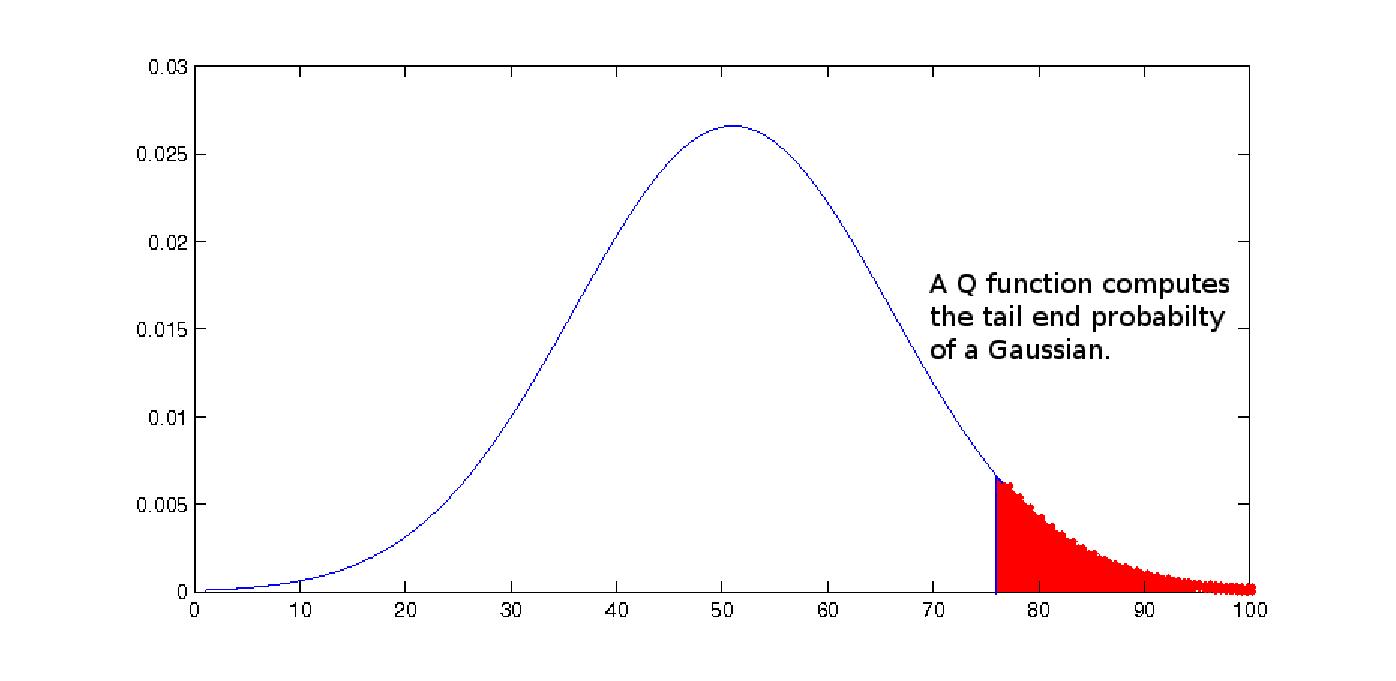
\includegraphics[scale=0.7]{qfunc.eps}\\
\caption{Tail of a Gaussian distribution.}\label{fig:qfunc}
\end{figure}

\noindent
We can define the Q function as the following:
\begin{equation}
Q(x) = {1\over{2}}\left(1 - \mathrm{erf}\left({x \over {\sqrt{2}}}\right)\right),
\end{equation}
where $\mathrm{erf}(x)$ is the error function.
Thus, instead of working out the mathematics, a communications engineer would instead refer to a look-up table for the value of $Q(x)$. Several key values of the
Q function include:
\begin{displaymath}
\centering
Q(-\infty) = 1 \hspace{10mm} Q(0) = 0.5 \hspace{10mm} Q(\infty) = 0
\end{displaymath}
Tables of Q function values can be found from the book by Abramowitz
and Stegun~\cite{abramowitz65}. For more information about Q
function, please refer to Section 4.2 of the course
textbook~\cite{rice2009}.

\subsection{Power Spectral Density}
To analyze a signal in the frequency domain, the power spectral density (PSD), $S_{x}(f)$, is often used to characterize the signal, which is obtained
by taking the Fourier Transform of the autocorrelation $R_{x}(\tau)$ of the signal $X(t)$.  The PSD and the autocorrelation of a function, $R_{x}(\tau)$,
are mathematically related by the Einstein-Wiener-Khinchin (EWK) relations, namely:
\begin{equation}
S_{x}(f) = \int_{-\infty}^{\infty} \! R_{x}(\tau)e^{-j2{\pi}f\tau} \, d\tau
\end{equation}
\begin{equation}
R_{x}(f) = \int_{-\infty}^{\infty} \! S_{x}(\tau)e^{+j2{\pi}f\tau} \, df
\end{equation}

\noindent
Using the EWK relations, we can derive some general properties of the power spectral density of a stationary process:
\begin{itemize}
\item $S_{x}(0)=\int_{-\infty}^{\infty} \! R_{x}(\tau)d\tau$
\item $E\{X^2(t)\}=\int_{-\infty}^{\infty} \! S_{x}(f)df$
\item $S_{x}(f)\geq 0$ for all $f$
\item $S_{x}(-f)= S_{x}(f)$
\item The power spectral density, appropriately normalized, has the properties usually associated with a probability density function:
\begin{equation}
p_{x}(f)=\frac{S_{x}(f)}{\int_{-\infty}^{\infty} \! S_{x}(f)df}
\end{equation}
\end{itemize}

\noindent
Using $H(f)$ to denote the frequency response of the system, we can relate the power spectral density of input and output random processes by the following equation:
\begin{equation}
Y(f)=|H(f)|^2 X(f),
\end{equation}
where $X(f)$ is the PSD of input random process and $Y(f)$ is the PSD of output random process.\\

\noindent For more information about power spectral density, please
refer to Section 4.4 of the course textbook~\cite{rice2009}.
\end{comment}


\newpage
\section{Additional Probability Simulation Experiments}
The MATLAB software uses a matrix language, which means it is
designed for vector and matrix operations. You can often speed up
your code by using vectorizing algorithms that take advantage of
this design. \textit{Vectorization} means converting \texttt{for}
and \texttt{while} loops to equivalent vector or matrix operations.
In this laboratory, MATLAB is used as a digital communication system
design and evaluation tool.  Due to the nature of many the
mathematical operations used in communications, it is also important
to
vectorize operations in MATLAB as much as possible.  Avoiding loops will save you many computational cycles and ultimately result in much shorter simulation times.\\

\noindent
Read the online documentation \textit{\textcolor{blue}{\href{http://www.mathworks.com/help/techdoc/matlab_prog/f8-784135.html}{Techniques for Improving Performance}}}
for more information about vectorization, as well as some other techniques for improving performance.

\subsection{Random Number Generators}
We will now focus on the generation of additive Ricean noise via the
manipulation of uniform and Gaussian random number generators. The
goal of this laboratory exercise is to refresh your knowledge about
probability and prepare you for conducting communication simulations
in MATLAB.

\subsubsection{Generation Process}
Generate two uniform random variables, x = $\{x_1, x_2, ...x_n\}$ and y = $\{y_1, y_2,...y_n\}$, on the interval [0,1].
Use \texttt{rand()} function of MATLAB. Let $n$ = 20,000.

\subsubsection{Random Variable Transformation}
Apply the following transformations to obtain two new random variables, $x_{std-normal}$ and $y_{std-normal}$:\\
\begin{equation}
x_{std-normal}=\mu_1+\sqrt{-2log(x)}cos(2 \pi y)
\end{equation}
\begin{equation}
y_{std-normal}=\mu_2+\sqrt{-2log(x)}sin(2 \pi y)
\end{equation}
\noindent
where $\mu_1$ and $\mu_2$ are equal to zero. Plot the histograms of $x_{std-normal}$ and $y_{std-normal}$. Describe and explain your observations.

\subsubsection{New Random Variables}
\label{sec:newrv}
Apply the following transformation to obtain a new random variable, $z_{rayleigh}$:
\begin{equation}
z_{rayleigh}=\sqrt{x_{std-normal}^2+y_{std-normal}^2}
\end{equation}
Make $\mu_1$=1 and $\mu_2$=2 and apply the same transformation to obtain another random variable, $z_{rician}$:
\begin{equation}
z_{rician}=\sqrt{x_{std-normal}^2+y_{std-normal}^2}
\end{equation}
Plot the histograms of $z_{rayleigh}$ and $z_{rician}$. Describe and explain your observations.

\subsubsection{Noise Generation}
We will now use the random variables $x$$_{std-normal}$ (or $y$$_{std-normal}$) and
$z_{rayleigh}$ to simulate the performance of an idealized binary phase shift keying (BPSK) transceiver system generate a symbol vector consisting of 20,000 random ``1'' and ``-1'' values.\\

\noindent{\textbf{Additive Gaussian Noise:}} Add the elements of $x_{std-normal}$ to the symbol vector and round the obtained noisy
symbols to the nearest constellation point (i.e., ``1'' or ``-1''). Repeat the procedure by
generating zero mean Gaussian random variables of different variances. Use the
following variance values:
\begin{equation}
\sigma^2=\{0.1, 0.1259, 0.1585, 0.1995, 0.2512, 0.3162, 0.3981, 0.5012, 0.6310, 0.7943, 1\}
\end{equation}
for generating different Gaussian random variables. Note that a standard normal random
variable, i.e., zero mean and unit variance, can be converted to a random variable of
desired mean $\mu_{desired}$ and variance $\sigma^2_{desired}$, namely x$\sim$ N($\mu_{desired}$, $\sigma^2_{desired}$), by the
transformation:
\begin{equation}
x=\mu_{desired}+\sigma_{desired}\times x_{std-normal}.
\end{equation}
Count the number of errors resulting for each value of the variance and generate a plot,
where the y-axis is the ratio of the number of errors to the total number of symbols
transmitted, while the x-axis consists of the variance values chosen. Use \texttt{semilogy()}
function from MATLAB. For the x-axis, use the vector obtained by converting each
element of the above variance vector into a vector N = 10*$log_{10}(1/\sigma^2)$. What do you observe?\\

\noindent{\textbf{Additive Rayleigh Noise:}} Now add the elements of ${z}_{rayleigh}$ to the symbol vector and round the obtained noisy
symbols to the nearest constellation point (i.e., ``1'' or ``-1''). Repeat the procedure by
generating Rayleigh random variables of different variances (use the Gaussian random
variables obtained previously and apply the procedure described in Section \ref{sec:newrv}.\\

\noindent
Count the number of errors resulting for each value of the variance and generate a plot,
where the y-axis consists of number of errors divided by the total number of symbols,
and the y-axis is the variance values chosen. Use \texttt{semilogy()} function from MATLAB. What do you observe?


\begin{comment}
\newpage
\section{Lab Report Preparation \& Submission Instructions}
Include all your answers, results, and source code in a laboratory
report formatted as follows:
\begin{itemize}
 \item Cover page: includes course number, laboratory title, names and student numbers of team, submission
 date.
 \item Table of contents, list of tables, list of figures.
 \item Pre-laboratory experiment (as an appendix).
 \item Responses to laboratory questions and explanation of
 observations.
 \item Responses to open-ended design problem.
 \item Source code (as an appendix).
\end{itemize}

Remember to write your laboratory report in a narrative approach, explaining your experience and observations in such a way that it provides the reader with some insight as to what you have accomplished.  Furthermore, please include images and outputs wherever possible in your laboratory report document.\\

\noindent Each group is required to submit a single report
electronically (in PDF format not exceeding 2MB) to
\texttt{alexw@ece.wpi.edu} by the scheduled due date and time.
Reports that do not meet these specifications will be returned
without evaluation and will receive a grade of ``0'' for the report
segment of the laboratory experiment.
\end{comment}

\newpage
\bibliographystyle{plain}
\bibliography{lab1bib}


\end{document}
